\cotefile{138}
\scanpage{46}
% archive sheet number: 45
Posons pour abréger $X=C_2$, soit $D$ le diviseur de ramification sur $X$ (de degré 6) -- son corps de décomposition est $\mathbb{Q}(i)$; \deleted{\unsure{soit|posons} $X^*=X\setminus D$}\inserted{posons $X^*=X\setminus D$}, \deleted{et soit $\widetilde X^*$ le rev. universel abélien de $X^*$}

Soit $X_\infty$ le \inserted{pro-}\unsure{revmt} \deleted{abélien}\inserted{principal} de $X$ défini par la famille des $\deleted{\unsure{C|X}}\unsure{X|C}_n$ ($n$ pairs), il a comme groupe $(\unsure{\mathbb{\Pi}|\Pi|\pi}_\infty)_{\deleted{X}\unsure{2|z}}$

\scanpage{47}
% archive sheet number: 46
\diagram{\resizebox{\linewidth}{!}{\begin{tikzcd}[ampersand replacement=\&,row sep=small,column sep=large]
X_n=\widehat{\mathrm{Spec}}\,k[x_n]\arrow[dd] \& \deleted{\unsure{x_n=}}x_{\unsure{m|n}}^{n}=x_1\\
(\vphantom{\dfrac11} \& \left)\vphantom{\dfrac11}\right.\ \boxed{\begin{array}{ccc}
n&\left\{\begin{array}{c}1\\1\\ \vdots\\1\end{array}\right.&n\end{array}}\ \bigg)\\
X_1=\widehat{\mathrm{Spec}}\,k[x_1=\deleted{\unsure{\zeta}}z]\arrow[dd] \&\\
(\vphantom{\dfrac11} \& \bigg)\ \boxed{\begin{array}{ccc}
\raisebox{-.5ex}{$2$}&\raisebox{-.5ex}{$2$}&1\\&&1\end{array}}\ \bigg)\\
X_0=\widehat{\mathrm{Spec}}\,k[\deleted{\unsure{x}}u] \&
\deleted{\unsure{x}}u=\frac12-\frac14(\deleted{\unsure{x}}z+\deleted{\unsure{x}}z^{-1})
\end{tikzcd}}}

\figure{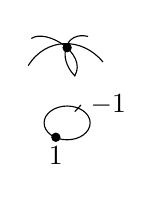
\begin{tikzpicture}[scale=.65]
\draw (-.7,1.1) .. controls (-.4,1.3) and (.4,.8) .. (.15,.37) .. controls (-.2,.72) and (-.04,1.25) .. (.41,1.14);
\draw (-.76,.57) .. controls (-.41,1.13) and (.3,1.13) .. (.7,.64);
\fill (0,.92) circle (2.6pt);
\draw (0,-.55) ellipse (.45 and .33);
\fill (-.22,-.83) circle (2.6pt) node[below] {$1$};
\draw (.15,-.33)--(.27,-.2) node[right] {$-1$};
\end{tikzpicture}}

ramification en dessous des p\textsuperscript{ts} $0,\infty$ (où la ramification est $n$)

p\textsuperscript{ts} de ramification en haut : $0,\infty$

ramification au dessus de

\[
\begin{aligned}
0&\ \deleted{\unsure{\infty\ \text{en haut}}\ (\unsure{\text{pt en dessus}|\text{pts en dessus}}}\inserted{(z=1,\ \text{ramification }2)}\\
1&\ \deleted{\unsure{\text{idem}}}\ (z=-1,\ \text{ramification }2)\\
\infty&\ (0\text{ et }\infty\ \text{ramification }1)
\end{aligned}
\]

\[
\mathbb{D}_\infty=(\mathbb{Z}_{/2})\mathbin{\underset{1/2}{\cdot}}\mu_\infty
\]

\diagram{\resizebox{\linewidth}{!}{\begin{tikzcd}[ampersand replacement=\&,column sep=small,row sep=large]
{\overset{0}{\bullet}\,(n)}\arrow[d] \& \& {\bullet\,\infty\,(n)}\arrow[d] \& {\bullet\,1\ (1)}\arrow[d,"{n\ \text{fois}}" {description,draw,ellipse,inner sep=1pt}] \& {\deleted{\unsure{-1}\ (1)}}\arrow[d,"{\deleted{\diagdown\!\diagdown}}" description] \& \\
0\ (1)\arrow[dr] \& \& \infty\ (1)\arrow[dl,dash] \& 1\ (2)\arrow[d,dash] \& {-1\ \deleted{\unsure{4\,(2)|4\ \text{fois}}}\ (2)}\arrow[d] \& \text{$n$ pair}\\
\& {\bullet\,\infty} \& \& 0 \& 1
\end{tikzcd}}}

\diagram{\begin{tikzcd}[ampersand replacement=\&,column sep=small,row sep=small]
\& \& \bullet\;\infty_1\ (1)\\
\overset{\bullet}{0\,(2)}\&\overset{\bullet}{1\,(2)}\&\bullet\;\infty_2\ (1)\\
\overset{\circ}{0}\&\overset{\cdot}{1}\&\overset{\cdot}{\infty}
\end{tikzcd}}

\figure{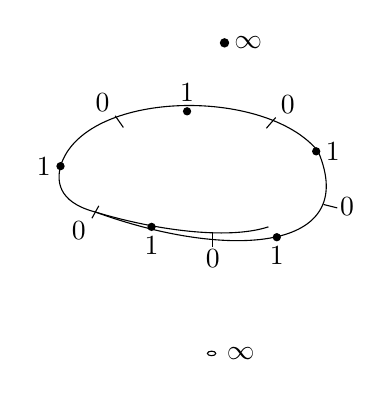
\begin{tikzpicture}[x=.82cm,y=.82cm]
\draw (-2,0) .. controls (-1.64,1.18) and (1.17,1.24) .. (1.99,.23) .. controls (2.65,-1.33) and (.6,-1.46) .. (-1.46,-.71) .. controls (-2.07,-.55) and (-2.05,-.2) .. (-2,0);
\draw[thin] (-1.46,-.71) .. controls (-.57,-.98) and (.57,-1.15) .. (1.22,-.94);
\foreach \x/\y/\a in {-2/0/left,-.04/.85/above,1.96/.23/right,-.59/-.94/below,1.35/-1.1/below}{\fill (\x,\y) circle (1.5pt) node[\a] {$1$};}
\foreach \x/\y/\a/\r in {-1.09/.69/above left/35,1.26/.67/above right/-41,-1.46/-.71/below left/-29,.36/-1.14/below/0,2.18/-.62/right/76}{\draw[shift={(\x,\y)},rotate=\r] (0,-.11)--(0,.11); \node[\a] at (\x,\y) {$0$};}
\fill (.54,1.91) circle (1.7pt) node[right] {$\infty$};
\draw (.34,-2.9) ellipse (.065 and .035) node[right,xshift=2pt] {$\infty$};
\end{tikzpicture}}

% printed form
% Upside-down typed address label.
\begin{center}\rotatebox{180}{\shortstack[l]{MR LE PROFESSEUR GROTHENDIECK A.\\MATHEMATIQUES\hspace{4cm}5}}\end{center}

\scanpage{48}
% archive sheet number: 47
% letterhead
ACADEMIE DE MONTPELLIER\\
\texttt{-{}-{}-{}-{}-{}-{}-{}-{}-{}-}\\
JC/JV

LE RECTEUR DE L'ACADEMIE DE MONTPELLIER\\
Chancelier des Universités

VU\quad la loi N° 68-978 du 12 novembre 1968 d'orientation de l'enseignement supérieur et notamment son article 18

VU\quad la démission présentée par M. le Professeur Jacques ROUZAUD, administrateur provisoire de l'Université de MONTPELLIER II

\begin{center}A R R E T E\\
\texttt{-{}-{}-{}-{}-{}-{}-{}-{}-{}-{}-}\end{center}

\uline{Article premier}.

La démission de M. le Professeur Jacques ROUZAUD de ses fonctions d'administrateur provisoire de l'Université de Montpellier II est acceptée à compter du 26 juin 1978 et l'arrêté rectoral du 15 décembre 1977 est abrogé à la même date.

\uline{Article deux.}

Monsieur Yvan MEYERHOEFFER, Conseiller du Tribunal Administratif de Montpellier, est chargé des fonctions d'administrateur provisoire de l'Université de Montpellier II à compter du 27 juin 1978 et jusqu'à la date d'installation d'un président élu.

Fait à Montpellier, le \handwritten{27 \unsure{Juin|juin} 1978}\\
LE RECTEUR,\\
\figure{
\begin{tikzpicture}[baseline=(signature.base)]
\node[inner sep=1pt,rotate=10] (signature) {\handwritten{\unsure{Richard}}};
\draw (-.60,-.17)--(-.74,.31)--(.43,.55);
\draw[->] (.66,.35)--(.68,-.04) .. controls (.24,-.09) and (-.51,-.32) .. (-.80,-.49);
\end{tikzpicture}}

\uline{Diffusion} : liste D\\
n° 4027\\
MONTPELLIER, le 27 Juin 1978

\scanpage{49}
% archive sheet number: 48
\[
\begin{aligned}
z'&=z^3\\
y'&=y(y^2-3x^2)\\
x'&=-x(x^2-3y^2)
\end{aligned}
\]

\[
\begin{aligned}
&z^6+y^2(y^4+9x^4-6x^2y^2)+x^2(x^4+9y^4-6x^2y^2)\\
&=x^6\unsure{+|-}y^6+z^6+\deleted{\unsure{9}}3x^2y^2(x^2+y^2)=\deleted{(x^2+y^2+z^2)^3}\\
&=x^6+y^6+z^6-3x^2y^2z^2
\end{aligned}
\]

\[
\left(\frac yz\right)^2+\left(\frac xz\right)^2=-1
\qquad x^6+y^6+z^6+
\]
\[
\begin{aligned}
& a\unsure{+|-}ib \qquad \deleted{a^2+b^2=-1}\\
\deleted{x^2+y^2+z^2}&\qquad\deleted{x^6+y^6+\unsure{3|z}}
\end{aligned}
\]

\diagram{\begin{tikzcd}[ampersand replacement=\&,column sep=small,row sep=small]
0\arrow[rr,bend left] \& \&0\\
1\quad {-1}\quad {\unsure{\mathcal X_2|X_2|X\,2}}\arrow[rr,bend right=15]\arrow[rr,shift right] \& \&1\quad X'\arrow[dd,"n"]\\
\infty\arrow[rr,bend right]\arrow[d,dash] \& \&\infty\\
{} \& \& {}
\end{tikzcd}}

\[
\begin{aligned}
\frac{p(x)}{\unsure{q|Q}(x)}&=\lambda\\
p(x)-\lambda q(x)&=0\\
p'(x)-\lambda q'(x)&=0\\
\lambda&=\frac{p'}{q'}\qquad p-\frac{p'}{q'}q=0\\
(x^2)^n&=(\pm x^n)^2 \qquad
\frac{\deleted{\unsure{q}}az^2+bz+c}{\deleted{\unsure{z}}z^2}
\qquad\deleted{q'p-}\ p'q-q'p=0\\
&\qquad \unsure{:}\,2z(az^2+bz+c)-
\end{aligned}
\]

\scanpage{50}
% archive sheet number: 49
% letterhead
U N I V E R S I T E\\
DES SCIENCES ET TECHNIQUES\\
DU LANGUEDOC\\
\texttt{-{}-{}-{}-{}-{}-{}-{}-{}-{}-{}-{}-}\\
Service de la Scolarité\\
MR/GJ\\
Diffusion : Liste H\\
N°3548

MONTPELLIER, le 8 JUIN 1978

% printed form
\uline{AVIS DE SOUTENANCE D'UNE THESE DE DOCTORAT D'ETAT}

\uline{Nom et prénom de la candidate} : LINDHEIMER née MONNIER Arlette

\uline{Titre de la thèse} : Contribution à l'étude diffusiomètrique des électrolytes dans des solvants mixtes de constantes diélectriques variables.

\uline{Date, heure et lieu de soutenance prévus} :\\
1er JUILLET 1978 à 9 Heures 30 mn\\
Salle de cours n° 2, U.S.T.L.

\uline{Nom du Directeur de thèse} : Monsieur le Professeur B. BRUN

\uline{Désignation du laboratoire où la thèse est préparée} :\\
Laboratoire des Interactions moléculaires, U.S.T.L.

\uline{Résumé de la thèse} : Les coefficients de diffusion ioniques ont été mesurés à 25°C pour des électrolytes dissous dans des solvants mixtes dont les constantes diélectriques prenaient des valeurs différentes :

- soit élevées comme dans les mélanges eau-N-méthylpropionamide,

- soit faibles comme dans les mélanges eau-alcool et eau-éther.

Dans le premier cas, la loi étendue relative au coefficient de diffusion a été vérifiée jusqu'à 0,2M environ ; dans les autres cas la présence d'associations ioniques a été mise en évidence et les paramètres d'associations ont été obtenus dans le cadre du modèle des paires d'ions.

\uline{Durée approximative des recherches ayant abouti à la thèse} : 5 ans

\uline{Noms des Rapporteurs} :

\diagram{\begin{tabular}{@{}l p{.70\linewidth}@{}}
SANFELD A. & Professeur, Chimie Physique, Univ. BRUXELLES\\
TURQ P. & Chargé de Cours, Chimie Physique, Univ. PARIS\\
BRUN B. & Professeur, Chimie Physique, U.S.T.L.
\end{tabular}}

\uline{Composition du jury} :

\diagram{\begin{tabular}{@{}l p{.70\linewidth}@{}}
BRUN B. & Professeur, Chimie Physique, Univ. Sciences et Techn. Languedoc MONTPELLIER\newline (Président)\\
SANFELD A. & Professeur, Chimie Physique, Univ. BRUXELLES\\
TURQ P. & Chargé de Cours, Chimie Physique, Univ. PARIS\newline (Membre extérieur choisi en raison de sa compétence scientifique)\\
GROMB S. & Professeur, Chimie Physique, U.S.T.L.\\
GIRAL L. & Professeur, Chimie Organique,U.S.T.L.\newline (Membre étranger à la spécialité de \unsure{:la|la} candidate)
\end{tabular}}

Le Secrétaire Général,\\
\handwritten{
\begin{tikzpicture}[baseline=-.2ex,x=1cm,y=1cm]
\node at (1.95,.28) {\unsure{E S}};
\draw (.05,-.09) .. controls (-.42,-.16) and (1.64,.53) .. (2.67,.62);
\draw (.05,-.09) .. controls (.34,-.13) and (3.65,.45) .. (2.65,.42) -- (2.13,.39);
\end{tikzpicture}}\\
\uline{E. SIAU}

% printed form
MR LE PROFESSEUR GROTHENDIECK A.\\
MATHEMATIQUES\hspace{4cm}5

\scanpage{51}
% archive sheet number: 50
\[
\begin{aligned}
\cos 2u&=\frac{1-\operatorname{tg}^2u}{1+\operatorname{tg}^2u}\\
\sin 2u&=\frac{2\operatorname{tg}u}{1+\operatorname{tg}^2u}
\end{aligned}
\qquad
\left\{\begin{aligned}x&=\frac{1-t^2}{1+t^2}\\y&=\frac{2t}{1+t^2}\end{aligned}\right.
\]
\[
\begin{aligned}
2\sin u\cos u&=2\underline{\cos^2u}\operatorname{tg}u=\\
t&=y/x\qquad\text{quand }z=1\\
&\deleted{\unsure{1+t^4+2t^2}}\\
t&=0
\end{aligned}
\]
\[
\begin{aligned}
x=1-t^2\qquad &y=2t\qquad z=1+t^2\\
&\deleted{y\qquad t=\pm i}
\end{aligned}
\]
\[
\begin{aligned}
z=0\quad\text{i.e.}\quad t=\mp i&\ \longrightarrow\quad x=2,\ y=\mp2i\quad\unsure{\sim|-}\quad x=1\quad y=\mp i\\
&\hphantom{\ \longrightarrow\quad x=2,\ y=\mp2i}\quad\sim\quad x=\pm i\quad y=1\\
y=0\quad\text{i.e.}\quad t=0&\qquad(1,0,1)
\end{aligned}
\]

\diagram{\begin{tikzcd}[ampersand replacement=\&,row sep=small,column sep=large]
{x^2+y^2+z^2=\deleted{\unsure{1}}0}\quad C_2=X\arrow[r] \& {\mathbb P^1=\widehat{\unsure{\mathrm{Sch}|\mathrm{Sp\acute ec}|\mathrm{Spec}}}(k[t])}\\
{(\pm i,1,0)}\arrow[r] \& t=\mp i\\
{(\pm i,0,1)}\arrow[r,arrows={Bar-}] \& t=0\qquad t=\dfrac yx
\end{tikzcd}}

\[
\begin{aligned}
x'&=1-t^2=1-\frac{y^2}{x^2}=\frac{x^2-y^2}{x^2}\\
y'&=2t=\frac{2y}{x}\qquad\text{ou}\quad (x',y',z')=(x^2-y^2,2xy,x^2+y^2\\
z'&=1+t^2=\frac{x^2+y^2}{x^2}
\end{aligned}
\]

\[
\left\{\begin{aligned}
x'&=x^2-y^2\\y'&=2xy\\z'&=x^2+y^2
\end{aligned}\right.
\qquad
\begin{aligned}
{x'}^2+{y'}^2-{z'}^2&=x^4+y^4-2x^2y^2\\
&\quad+4x^2y^2\\
&\quad\deleted{\unsure{+}}-(x^{\unsure{2|4}}+y^2)^2=0
\end{aligned}
\]

\diagram{\begin{tikzcd}[ampersand replacement=\&,column sep=large,row sep=small]
X\arrow[r,"2"]\arrow[dr,dash,bend right,"f_n"'] \& X'\arrow[r,"{n\ \text{impair}}"] \& X'\\
\& X\arrow[ur,"2"'] \&
\end{tikzcd}}

\[
\begin{aligned}
\unsure{t}\qquad s&=-\frac{\deleted{\unsure{z}}t+i}{t-i}=-\frac{(t+i)^2}{t^2+1}=-\frac{t^2-1}{t^2+1}-\frac{2it}{t^{\unsure{2|1}}+1}\\
\left(\frac{t+i}{t-1}\right)^{\unsure{n|4}}&=
\end{aligned}
\]

\scanpage{52}
% archive sheet number: 51
% letterhead
HARVARD UNIVERSITY\\
DEPARTMENT OF MATHEMATICS\\
\textsc{Area Code} 617\\
495--2170

\figure{
\begin{tikzpicture}[x=1cm,y=1cm,line join=round]
\draw (-.85,1.04)--(.85,1.04)--(.85,.37) .. controls (.85,-.16) and (.49,-.77) .. (0,-1.02) .. controls (-.51,-.76) and (-.85,-.16) .. (-.85,.37)--cycle;
\foreach \x/\y/\a/\b in {-.41/.50/V/E,.40/.50/R/I,0/-.30/T/S}{
\begin{scope}[shift={(\x,\y)}]
\draw (-.30,-.23) rectangle (.30,.23);
\draw (-.25,-.18)--(-.23,.25)--(-.05,.24)--(0,.21)--(.05,.24)--(.24,.24)--(.25,-.18)--(.05,-.18)--(0,-.21)--(-.06,-.18)--cycle;
\draw (0,.21)--(0,-.20);
\foreach \s in {-1,1}{\draw (\s*.29,.17)--(\s*.36,.14)--(\s*.36,.09)--(\s*.29,.07); \draw (\s*.29,-.09)--(\s*.34,-.12)--(\s*.34,-.17)--(\s*.29,-.18);}
\node[inner sep=0,font=\tiny] at (-.12,0) {\a};\node[inner sep=0,font=\tiny] at (.12,0) {\b};
\end{scope}}
\node[inner sep=0,font=\tiny] at (0,-.30) {A};
\end{tikzpicture}}

\textsc{Science Center}\\
\textsc{One Oxford Street}\\
\textsc{Cambridge, Massachusetts} 02138

June 10, 1978\\

Dear Friend,\\

This letter concerns the 80th birthday of Oscar Zariski. This will take place on April 24th, 1979. I have been talking to Jun-Ichi Igusa, who together with Jerry Sampson has recently taken over the Editorship of the \uline{American} \uline{Journal} \uline{of} \uline{Mathematics}, and they agreed that it would be a fine thing to dedicate one (and perhaps two) issue(s) of the \uline{American} \uline{Journal} to Oscar on this occasion. I'm sending this letter out to about thirty of his friends, colleagues and students to ask if they would like to dedicate a paper to Oscar in this issue. Unfortunately, as you can guess from the date of his birthday, we can only do this by adhering to a strict deadline. I sincerely apologize for launching a project like this at such a late date and must take full blame for this myself. However, the upshot is that the absolute deadline for contributions must be November 1st (or January 1st, \uline{if} \uline{we} \uline{get} \uline{enough} \uline{submissions} \uline{for} \uline{a} \uline{second} \uline{issue}): The issue(s) will then be the first one (or first two) of the \uline{American} \uline{Journal} in 1979.

I will be very pleased if you find it possible to send me a paper for Oscar's 80th birthday. But I fully understand if the short notice makes this impossible. In any case, to help in our planning I would be very grateful if you would drop me a line now indicating whether or not you expect to be in a position to send us a manuscript, and, if so, roughly what length it might be. (We have a maximum of 460 printed pages to use and if we are deluged there is a small chance that we may have to limit the length of individual submissions.) Please write me at:\\
Wallston Road\\
Tenants Harbor, Maine\quad 04860\\
U.S.A.\\

where I will be until about September 10th.

Best regards,\\
\handwritten{\unsure{David Mumford}/mjm}\\
David Mumford\\

DM/mjm

\scanpage{53}
% archive sheet number: 52
\[
\unsure{\Pi|\mathbb{\Pi}|\pi}_n=\mu_n^3/\mu_n
\qquad
\begin{aligned}
0'\unsure{=|\sim|\mapsto}\infty'',\quad 1'&=0'',\quad \infty'=\infty''\\
\underbrace{0'=1'},\quad&\underbrace{1'=\infty'}\quad ?
\end{aligned}
\]

\diagram{\resizebox{\linewidth}{!}{\begin{tikzcd}[ampersand replacement=\&,font=\scriptsize,row sep=1.2em,column sep=.8em]
\& \& \& \& {\widetilde X(p,q,r;\,n)}
 \arrow[dlll,"\Pi_n"']\arrow[dddlll,"{\mu_p\times\mu_q\times\mu_r\times\Pi_n}" description]
 \arrow[dd,leftrightarrow,"{\mu_p\times\mu_q\times\mu_r}"]
 \arrow[dddddllll,bend left=65,leftrightarrow,""{name=outerjoin,coordinate,pos=.67},"{\mu_{2p}\times\mu_{2q}\times\mu_{2r}\times\Pi_n}" description]\\
\& {\widetilde X_2(p,q,r)=X_2(2p,2q,2r)}\arrow[dd,"{\mu_p\times\mu_q\times\mu_r}"] \& \& \&\\
{X_2(p,q,r)}\arrow[ddd,"{\mu_p\times\mu_q\times\mu_r}"'] \& \& \& \& {\widetilde X_2(n)}
 \arrow[dlll,"\Pi_n"']\arrow[d,"{\unsure{\mu_2|\mu_{2n}}}"]\\
\& {X_2(2,2,\unsure{2|6})=\widetilde X_2}
 \arrow[ddl,"{\mu_2^3}" description]\arrow[dr,"\mu_2"] \& \& \& {X_{4n}}\arrow[dll,"\Pi_n"']\\
\& \& X_4\arrow[dll,"\Pi_2"']\arrow[ddll,bend left=15,"\Pi_4"] \& \&\\
X_2\arrow[d,"\Pi_2"'] \& \& \& {\deleted{\unsure{\mu_{2p}\times\mu_{2q}}}\quad
\deleted{\unsure{\Pi_{2n}\;\mu_2^3\times\mu_{2n}}}} \&\\
X_1\arrow[to=outerjoin,bend right=25,"\Pi_{2n}"'] \& \& \& \&
\end{tikzcd}}}

Si $p=q=r=1$, $n=2$ on trouve
\[
\mu_2\times\mu_2\times\mu_2\times\underbrace{\Pi_2}_{\mu_2^3/\mu_2}
\]
TSVP

\scanpage{54}
% archive sheet number: 53
\diagram{\begin{tikzcd}[ampersand replacement=\&,column sep=small]
\widetilde X_2\arrow[dr] \& {}\arrow[l,very thick] \&\\
\&X_4 \& {\deleted{\unsure{C|X}}X_8}\arrow[l]
\end{tikzcd}}

% letterhead
% Printed upside down relative to the diagram.
\begin{center}\rotatebox{180}{\shortstack{UNIVERSITÉ DES SCIENCES\\
ET TECHNIQUES DU LANGUEDOC\\
\rule{1.1cm}{.3pt}\\
INSTITUT DE MATHEMATIQUES\\
Place Eugène Bataillon\\
34060 MONTPELLIER CEDEX\\
\rule{1.1cm}{.3pt}}\qquad\shortstack{Montpellier, le}}\end{center}

\scanpage{55}
% archive sheet number: 54
\[
X=\frac{y^2-x^2}{z^2}\qquad Y=-\frac{2xy}{z^2}
\]
\[
X+iY=\frac1{z^2}(y^2-x^2-2ixy)=\frac1{z^2}(y\deleted{\unsure{+}}\unsure{-|+}ix)^2
\]
\[
\begin{aligned}
(X+iY)^n&=\frac1{z^{2n}}(y-ix)^{2n}=\frac1{z^{2n}}\bigl(P_n(x,y)+iQ_n(x,y)\bigr)\\
&\overset{?}{=}\frac{{y'}^2-{x'}^2}{{z'}^2}\deleted{\unsure{+}}\unsure{-|+|\mp}2i\frac{x'y'}{{z'}^2}
\end{aligned}
\]

$x',y',z'$ fonctions rat des $x,y,z$ ?? P.ex. $z'=z^n$

\[
\begin{aligned}
\deleted{P_n(x,y)=}\quad&\frac{\deleted{\unsure{A}}\unsure{B|A}_n(x,y,z)}{\deleted{\unsure{z|Z}}z^n}\quad\text{et}\quad B_n\\
&\deleted{\unsure{A}}B_n(x,y)^2-A_n(x,y)^2=P_n(x,y)\\
&-2\deleted{\unsure{B}}A_n(x,y)B_n(x,y)=Q_n(x,y)
\end{aligned}
\]

\[
X+iY=\left(\frac{y-ix}{z}\right)^2=\left(\frac yz-i\frac xz\right)^2
\]
\[
\Bigl(\frac yz\unsure{=|-}i\frac xz
\qquad \left(\frac yz-i\frac xz\right)^{2n+1}
\]
\margin{$(-i)^3=-i(i^{\unsure{2|1}})=i$}
\[
\begin{aligned}
\left(\frac yz-i\frac xz\right)^3&=\frac1{z^3}
\underbrace{\bigl[y^3\deleted{\unsure{+}}-3iy^2x\deleted{\unsure{+}}-3yx^2+ix^3\bigr]}_{y^3-3yx^2+i(x^3-3y^2x)}\\
&\qquad y(y^2-3x^2)+ix(x^2-3y^2)
\end{aligned}
\]

\scanpage{56}
% archive sheet number: 55
% letterhead
U N I V E R S I T E\\
DES SCIENCES ET TECHNIQUES\\
DU LANGUEDOC\\
\texttt{-{}-{}-{}-{}-{}-{}-{}-{}-{}-{}-{}-}\\
Service de la Scolarité\\
MR/GJ\\
Diffusion : Liste H\\
N° 3758

MONTPELLIER, le 15 Juin 1978

% printed form
\uline{AVIS DE SOUTENANCE D'UNE THESE DE DOCTORAT D'ETAT}

\uline{Nom et prénom du candidat} : WALTER Philippe

\uline{Titre de la thèse} : Recherches écologiques et biologiques sur les Scarabéides Coprophages d'une savane du Zaïre.

\uline{Date, heure et lieu de soutenance prévus} : 3 JUILLET 1978 à 9 Heures 30 mn\\
Salle de cours n° 6, U.S.T.L.

\uline{Nom du Directeur de thèse} : Monsieur le Professeur Renaud PAULIAN.

\uline{Désignation du laboratoire où la thèse est préparée} : Zoologie (Professeur LEGENDRE)

\uline{Résumé de la thèse} : Les recherches ont été effectuées sur le Plateau Bateke zaïrois. Les résultats sont présentés en trois parties :

1) le peuplement (composition d'ensemble, aspects biogéographiques, répartition dans les différentes formations végétales, fluctuations des densités de population, sex-ratio)

2) observations autoécologiques et biologiques (préférences trophiques, heures d'activité, éthologie)

3) morphologie larvaire : description détaillée de 12 larves.

\uline{Durée approximative des recherches ayant abouti à la thèse} : 5 ans 1/2.

\uline{Noms des Rapporteurs} :

\diagram{\begin{tabular}{@{}l p{.70\linewidth}@{}}
PAULIAN R. & , Professeur, Zoogéographie, Rectorat BORDEAUX\\
LAMOTTE M. & , Professeur, Ecologie, Ecole Normale Supérieure PARIS\\
LEGENDRE R. & , Professeur, Zoologie Ecologie, U.S.T.L.
\end{tabular}}

\uline{Composition du jury} :

\diagram{\begin{tabular}{@{}l p{.70\linewidth}@{}}
LEGENDRE R. & , Professeur, Zoologie Ecologie, U.S.T.L.\newline (Président)\\
PAULIAN R. & , Professeur, Zoogéographie, Rectorat BORDEAUX\\
LAMOTTE M. & , Professeur, Ecologie, Ecole Normale Supérieure PARIS\newline (Membres extérieurs choisis en raison de leur compétence scientifique)\\
EUZET L. & , Professeur, Parasitologie, U.S.T.L.\newline (Membre étranger à la spécialité du candidat)\\
LUMARET J.-P. & , Maître-assistant, Biogéographie, Univ. MONTPELLIER III.\\
BARAUD J. & ., Professeur, Biochimie, Univ. BORDEAUX
\end{tabular}}

Le Secrétaire Général,\\
\handwritten{
\begin{tikzpicture}[baseline=-.2ex,x=1cm,y=1cm]
\node at (1.86,.37) {\unsure{E Siau}};
\draw (.04,-.12) .. controls (-.28,-.16) and (1.64,.42) .. (2.70,.59);
\draw (.04,-.12) .. controls (.43,-.20) and (3.60,.55) .. (2.78,.53) -- (2.30,.50);
\end{tikzpicture}}\\
\uline{E. SIAU}

\scanpage{57}
% archive sheet number: 56
\begin{flushright}autom. des\\groupoïdes\end{flushright}

\scanpage{58}
% archive sheet number: 57
\uline{Automorphismes de groupoïdes.}

1) \unsure{Soient|Soit} $C$ \deleted{$\unsure{=(C_0,C_1,\ldots)}$} un groupoïde, $C'$ une catégorie, on s'intéresse à
\[
\operatorname{Hom}(C,C')=\operatorname{Ob}\,\underline{\operatorname{Hom}}(C,C').
\]
On a
\[
\operatorname{Hom}(C,C')\longrightarrow\operatorname{Hom}(\underbrace{\operatorname{Ob}C}_{C_0},\underbrace{\operatorname{Ob}C'}_{C'_0})
\]
Soit
\[
f_0:C_0\longrightarrow C'_0
\]
on cherche les $f\in C\longrightarrow C'$ qui lui donnent naissance. On trouve\unsure{:}

\uline{Proposition} a) Pour qu'il existe un $f$ au dessus de $f_0$, il f. et il s. que pour $x,y\in C_0$ appartenant à la $=$ comp. connexe de $C$ (i.e. tels que $\operatorname{Hom}_C(x,y)\ne\varnothing$) on ait $f_0(x)\simeq f_0(y)$. \deleted{b) \unsure{Supposons} cette condition satisfaite.} b) Pour tte composante connexe $C(i)$ de $C$, soit $a_i\in C(i)_{\deleted{\unsure{a}}0}$, et pour tt $x\in C(i)_0$, soit $u_x:a_i\xrightarrow{\sim}x$. Alors
\[
\resizebox{\linewidth}{!}{$\displaystyle\operatorname{Hom}_{f_0}(C,C')\xrightarrow{\sim}
\prod_{\deleted{\unsure{x\in C|x\in C_0}}C_0\setminus\{a_i\}}
\deleted{\unsure{\mathrm H|\mathrm I}}\operatorname{Isom}(f_0(a_{i(x)}),f_0(x))
\mathbin{\times}\prod_i\operatorname{Hom}(\operatorname{Aut}(a_i),\operatorname{Aut}(f_0(a_i$}
\]
% The second factor runs to the lower and right cut edges.

\scanpage{59}
% archive sheet number: 58
\[
\resizebox{\linewidth}{!}{$\displaystyle f\longmapsto\left(\bigl(\underbrace{f_{\deleted{\unsure{0}}}(u_x)}_{\ell_x}\bigr)_{x\in C_0},
\bigl(f_{a_i,a_i}:\underbrace{\operatorname{Aut}(a_i)\longrightarrow\deleted{\unsure{\operatorname{Aut}|)}}\operatorname{Aut}}_{\varphi_i}(f_0(a_i))\bigr)\right).$}
\]

c) Pour que $f$ soit \unsure{fidèle|fidèl}, il f et suffit que $\deleted{\unsure{\forall}}\forall i\in I$, $\varphi_i$ soit injectif.

Pour que $f$ soit pleinement \unsure{fidèle|fidèl}, il f et suffit que \deleted{\unsure{;}} 1°) pour $i\ne j$, on ait $\operatorname{Hom}(f_0(a_i),f_0(a_j))=\varnothing$

2°) pour $\deleted{\unsure{\forall i|\forall}}\ x,y\in {C_{(i)}}_0$,
\[
\deleted{\unsure{\operatorname{Hom}}}\operatorname{Isom}(f_0(x),f_0(y))\xrightarrow{\sim}\operatorname{Hom}(f_0(x),f_0(y))
\]

3°) $\forall i\in I$, $\varphi_i$ est un iso.

\deleted{d) \unsure{Soit} $C$}

Pour que $\deleted{\unsure{d}}f$ soit une équivalence, il f. et s. qu'on ait de plus

4°) Tout $x'\in C'_0$ est isomorphe à un des $f_0(a_i)$

Pour que $f$ soit un isom, il faut et s. qu'on ait 1°), 2°), 3°) et de plus

$4'$\textsuperscript{o}) $f_0$ bijective.

